\documentclass[]{article}
\usepackage{geometry}                
\geometry{letterpaper,tmargin=1in,bmargin=1in,lmargin=1in,rmargin=1in}
\usepackage[parfill]{parskip}
\usepackage{float}
\usepackage{url}
\usepackage{graphicx}
% Title Page
\title{Better Late Than Never: An Analysis of Unitrans's Delays}
\author{Wesley Brown, Curtis Lou, Sam Sridhara, Yi-Chun Chen}

\begin{document}
	\maketitle
	Repo Available at: \url{https://github.com/141bbusproggy/141b_bus_project}
	\pagebreak
	\section{Workload}
	Our workload was quite heavy for this project, as it required a significant amount of experimentation for parsing the badly formatted and documented UmoIQ API and Unitrans data. Curtis Lou spent roughly a week refining the scraper.ipynb to efficiently and reliably parse data; this involved first understanding the API documentation, making requests to various endpoints by hand to comprehend its output, adapting a Python script to the returned XML format, and finally refining the script by implementing multithreading and proper interfacing with Linux crontab, involving non-trivial amounts of trial-and-error validation and bug-fixes, to automate the process. In addition, he completed the introduction, part of the methods section, part of the results section, and overall  proofreading of the report. Wesley Brown worked diligently to clean and extract the important information from the raw files over the course of a few days. This involved utilizing Element Tree XML processing to parse the nested data and store the extracted results in a SQLite database; containing two tables: predictions and schedules. Additionally, he fixed merge issues that existed in the visualization code. Finally he wrote the part of the methods section focused on the parsing methodology. Sam Sridhara worked on visualizing the data utilizing matplotlib, and seaborn. He made multiple graphs, including bargraphs, heatmaps, and time series graphs. He got help from Wesley Brown who helped fix these graphs. Additionally Sam Sridhara wrote the abstract, summary, and results sections of the code. Yi-Chun Chen produced several visualizations, wrote analysis for the graphs, and assisted with proofreading the final report. 
	\section{Abstract}
	This study hopes to analyze the Unitrans bus arrival reliability by comparing schedule data to actual arrival times. XML files for schedules and arrivals were scraped from a third-party provider for Unitrans, parsed, and then merged. Lateness was calculated by subtracting the arrival time that was scheduled by the system with the arrival times that were scraped. The data was analyzed using Python, SQL, and pandas to examine patterns in lateness. The visualizations are consistent with the bus line performances being generally early or on time and on very rare occasions being late by a few minutes. The time series graph and heatmaps also indicate that general performance of the lines remain consistent throughout the days and hours of the week that was scraped. Overall, we can state that the bus system is generally reliable and is mainly on time or earlier than what was scheduled, and follows a consistent schedule that does not deviate.
	\section{Introduction}
	The Unitrans system is the sole means of off-campus transport for countless students at UC Davis. It must be sufficiently dependable in order to guarantee that students are able to arrive on campus to attend classes in a timely manner. However, both the continually aging infrastructure of the city of Davis and ever growing student body of UC Davis strain the bus system's ability to maintain its reliability. We aim to analyze the problem of Unitrans's tardiness; we aim to identify both peak hours necessitating extra support and bus lines facing potentially insufficient resources or obstacles inhibiting their ability to meet demand.
	
	By intercepting the network flow of existing UC Davis bus information sites, we were able to identify a scrapable API operated by UmoIQ providing both arrival and schedule information. Given the large number of stops (over 200), we opted to record both datasets for only the main terminus stations at the Silo and Memorial Union every 5 minutes starting from 6AM to 11PM, which is the operating hours provided by the university.
	
	We collected the variables of both daily planned schedules for all lines and live arrival times for bus arrivals. The former dataset described the pre-determined expected time of arrival for all buses, assuming no disturbances due to traffic. The latter included up-to-date information regarding the arrival's line, expected time of arrival, vehicle number, and direction. Therefore, by differencing the expected and actual arrival times, we would be able to identify the quantity and frequency of delay, as well as correlations between lines and delays.
	
	Our daily scraping generated approximately over 1000 files a day (roughly 60kB), before cleaning and condensing.
	Our approach will be to complete our goals in steps: we will scrape the raw data from the UmoIQ endpoint, interpret and load the data into an SQLite database, create graphs based on the database, and interpret the graphs to form our conclusions. We hypothesize that some lines will be regularly later or earlier than others (due to differences in route and equipment). We assume that bus schedules will not change from week to week, and that every route will be completed. 
	\section{Methods}
	Our project began with the collection of data from the UmoIQ API (scraper.ipynb), as the scraper would need to continuously collect data over the entire time span of the week. The scraper is composed of two different sections: one section retrieves the schedule, which would be done once, as we assumed it would not change, and the other section polls several APIs to retrieve the active predictions for each line at the terminus stations. Several design considerations were made regarding the scraper, especially as it was being run on a very limited-resource AWS instance. First, we opted to multithread the program, due to the risk of a single request taking significantly longer than others, potentially causing inconsistent timing on a single threaded system. In addition, we opted to have a cronjob run the program every 5 minutes in the desired timespan of 6am to 11pm; the alternative would be to run the script as a daemon for a week while occasionally scraping the API. We did not believe the alternative solution to be reliable. According to researchers at the University of Massachusetts, Python’s memory usage is not negligible, with, “...the integer 1 consum[ing] 4 bytes in C, but 28 bytes in Python; ‘a’ consumes 2 bytes in C, but 50 bytes in Python…because garbage collection delays memory reclamation, it can further increase the amount of memory consumed compared to native code” (Berger, et.al). As we were unsure of whether the libraries we used contained any memory leaks, which would accumulate into system memory exhaustion from running for such an extended period, we chose the option of having the operating system run and terminate the process (thereby freeing the memory) as needed. This scraper used the requests library to download the raw XML response from multiple HTTP endpoints. Our scraping was designed in accordance with the API documentation from the UmoIQ PDF (provided in references); we included the ‘commands’ verb as part of the parameters of our request, and saved the files with a time and date format that would be conducive to our later data cleaning.
	In order to properly utilize our scraped data, significant effort was needed to transform it into a usable format. Our goal for this step was to organize and store them within a SQLite database, containing two tables: one for the permanent schedules and the other for the recorded predictions. 
	
	We started with the schedules first to procure a baseline for our analysis. Because our analysis depended on the deviations in lateness, having high quality schedule data was integral for our project. We began by using the ElementTree module to store each schedule XML file as a hierarchical tree. Because the stop names and tags were permanent attributes, we saved time by creating a map from the stop tags to their corresponding names. This allowed us to quickly apply this change to all the individual stops, without having to parse the data every time for them. Since the XML data followed a clear hierarchical structure, we were able to effectively loop through each route, each block within a route, and each stop within each block. At each layer, specific data remained constant, so we pushed data parsing as high up in the parsing stream as possible to avoid redundant calls. The only data that proved to not be useful was the epoch time, to our surprise. This is because our initial assumptions regarding the epoch time were incorrect; there was no proper documentation available regarding what the specific attributes of the data corresponded to. The ‘direction’ string attribute was set to lower case because there was a discrepancy in naming between the schedules and predictions. Additionally, the time variable was saved and stored into our database as a string; this was to avoid having to deal with the time being saved in conjunction with the Unix Epoch if it was saved as a date-time object. We also filtered out any schedules that did not have times associated with them. Finally, we subsetted the schedules data to only include the useful service classes (specific schedules for each day of the week) to only the regular weekday and weekends, as we were unsure what the other service classes represented. Each file in each route was scanned through by our parsing algorithm and saved to a local SQLite database table called schedules. 
	Parsing the predictions, as expected, ended up being the more difficult of the two. The initial setup was the same as with parsing the schedules using ElementTree on the XML files. The first issue with the predictions file was that buses do not run at the same times and frequencies every day. Therefore, many of the XML files have the proper frame, but no actual data within them. First, we ran an algorithm that involved scanning through each prediction block, grabbing the header attributes, then checking if the prediction block contained a valid direction tag. This was an indicator that bus prediction data had been recorded for that specific time. The main issue at this point was deciding what to do about each of the prediction entries within a direction block. We ultimately determined that all of the instances of observations after the first instance referred to later buses that would be captured again in other files. Since our goal was not to build a live bus tracker, we only needed to save the first entry to then be able to compare the lateness of that specific bus. Additionally, we used the filename which corresponded to the time at which the data was requested from the API, and combined it with the minutes until arrival data to determine the estimated time of arrival. All of the associated data with each stop was saved, apart from the epoch time, as we were no longer using the epoch time from schedules. The direction string attribute was also set to lower case here because there was a discrepancy in naming between the schedules and predictions. Additionally, a day of the week feature was extracted from the predicted arrival date-time, so that it could be used to assign and match to the service class in the schedule table. This algorithm was then applied to each file within each folder that was recorded over the week of scraping to clean and store it into a SQLite database table called predictions. 
	
	All our operations are deterministic, so we scanned through the database and confirmed by examining a subset of the documents to validate the data. Since there is no variation in the parsing process, the validation applies across the dataset.
	In order to make our two high quality data tables useful, we needed to merge them together. This proved to be the most difficult task. We first needed to compare the scheduled time which was stored as just a time, with the prediction time which was stored in a date-time formulation. We did this by subsetting the time information from the predicted date-time, subtracting it from the scheduled time, then multiplying it by 1440 to get the difference in minutes. Julian time was used to bridge the gap between performing math on standard dates in SQL, by converting it into a format that is easy to subtract. Furthermore, the vast number of combinations of stop recordings needed to be accounted for to only select ones that specifically matched the entry we were looking for. We performed an inner join on the two tables, combining on the route tag, stop tag, direction, block id, and service class. Then we filtered out the NULL prediction values. The resulting query result contains duplicate rows for each stop combination. In order to filter out the correct record, we sorted by the unique prediction ID and the absolute value of the lateness in ascending order. We then picked the first one that appeared, as that one matched the scheduled time the closest. 
	\section{Results}
	Through the filtering and merging of the tables, multiple graphs were created in order to visualize metrics that would make us understand the reliability of each of the different bus lines. In the “Top 15 Routes” graph (figure 1), we were able to see which routes have had a higher on-time performance rate than other lines. In the graph we can clearly see that the U Bus had the highest rate of being on-time with a percentage of over 85 percent, while the M, J, and D bus lines were following closely behind, with an average of over 80 percent. The worst performing buses would be the C, E, L, and Q buses with a 70 percent on-time rate. Most notably, none of these buses fell below the 60 percent margin of the on-time rate. It is clear that all of the lines are generally consistent with their time schedules, boasting an over 70 percent on-time rate.
	
	The “Rolling 60-minute Average Lateness Over Time” time series graph (figure 2) shows the performance over bus lines as an average over different days of the week. On average, Unitrans is consistently on time, deviating, in extreme cases, from 1.3 minutes early to over 1.5 minutes late. From the graph, it is apparent that the more significant time spikes of lateness occur on Monday, Wednesday, Thursday, and Saturday. These days have an average lateness of over 30 seconds to almost 90 seconds of delays. Overall, the time series analysis graph does indicate that the bus schedule does remain fairly consistent with some minute time differences, but no severe changes that would affect a passenger’s wait time to a noticeable amount.
	
	The “Overall Lateness Distribution” graph (figure 3) corroborates the findings of the time series graph. The bar graph, which is skewed right, suggests that most buses will arrive 1 minute early, with very few cases of buses arriving late. Most of the bus arrival record counts are populated around being one minute early, or the bus being on time. There are only a few instances of buses being more than a minute late, or the bus being late in any instance. From this we can conclude that in the time series graph that the spikes that were present can be considered outliers, and not an occurrence that happens extremely often.
	The “Average Lateness By Routes” graph (figure 4) shows the average lateness by route worst to best. The worst performing bus line, by far, is the F bus line with an average earliness of 10 seconds. The top 4 best bus lines in regards to earliness are the A, O, Z, Q reaching almost a minute of earliness. On average the bus lines exhibit an average earliness of about 30 seconds to 60 seconds.
	
	The “Average Bus Lateness Heatmap” graph (figure 5) indicates the days as the x-axis and the y-axis as the hours. The heatmap indicates that almost all of the bus lines are early to their stops when the whole Unitrans system’s reliability for all days and times is considered, with only a few instances of being late to their stop. In the worst case scenario (Wednesday), a passenger would have to wait 41.4 seconds over the expected time. Overall, the bus lines indicate that they are usually early to their stops, and are rarely late to their stop.
	
	Our “Average Bus Lateness by Route and Hour (All Days)” graph (figure 6) has the route as the y-axis and hour of day as the x-axis; this graph should show the consistency of the performance of a line across all days at a given time. While the majority of lines were in the bounds of being either 1 minute early or late across all times, the C line’s performance at 10pm was an anomaly at 20 minutes late. We initially believed that this was a bug. However, we investigated our dataset (figure 7) and discovered that there was indeed a strangely high rate of lateness (20-23 minutes) at that time for the C line. We are unsure of the cause of delay at such a late time (when traffic and demand should be light); it is possible that the driver of that line is simply ending service, but the arrival system is still recording. 
	
	Across these multiple different graphs, we believe that bus lines mostly follow a uniform pattern: they usually arrive earlier than scheduled, and are rarely late to stops. We hypothesize the buses are able to maintain this performance by arriving at stops early, allowing more room for them to make their next stop at the correct time. The most tardy bus arrivals are on weekdays; this could be attributed to the evening rush hours on those days. We postulate that the reason for the tardiness can be attributed to more students returning home during the evening, which can lead to overcrowding of buses causing delayed times. In addition, we theorize that stoplights are configured differently during this period, and there are more pedestrians walking around this period of time to return home. Overall, most buses have been observed arriving early at stops, except in rare cases.
	\section{Summary}
	Overall, the visualizations suggest that the bus service reliability is mostly consistent and stable throughout the week. The bus lines remained, for the most part, on schedule or slightly earlier than expected by 1 minute. Some routes, such as the C line, experienced anomalies which caused delays of up to 20 minutes; on average, the C and E routes may require further investigation to resolve potential obstacles to service, as their average performance is worse than other lines. This would likely involve a further inquiry with other tracking services, as our UmoIQ API has limited resolution for arrival times, and no data regarding road conditions or obstacles en-route. Other routes demonstrate more reliability than others. These routes, including the Z and A line were consistently on time or earlier than others. The heatmap and time series showed small fluctuations throughout most of the day, but peaks in lateness during evenings, and especially on Wednesday. This lines up with traditional “rush hour” behavior. For the most part, Unitrans remained consistent to the schedule or early. These findings indicate that the Bus Lines in UC Davis follow a strict and uniform schedule that is reliable, but require some improvements on certain routes and days of the week.
	\section{References}
	Berger, Emery D., Sam Stern, and Juan Altmayer Pizzorno. "Triangulating python performance issues with {SCALENE}." 17th USENIX Symposium on Operating Systems Design and Implementation (OSDI 23). 2023.
	
	“Public XML Feed.” NextBus XML Feed, 18 May 2021, \url{retro.umoiq.com/xmlFeedDocs/NextBusXMLFeed.pdf}. 
	\section{Figures and Tables}
	\begin{figure}[H]
		\centering
		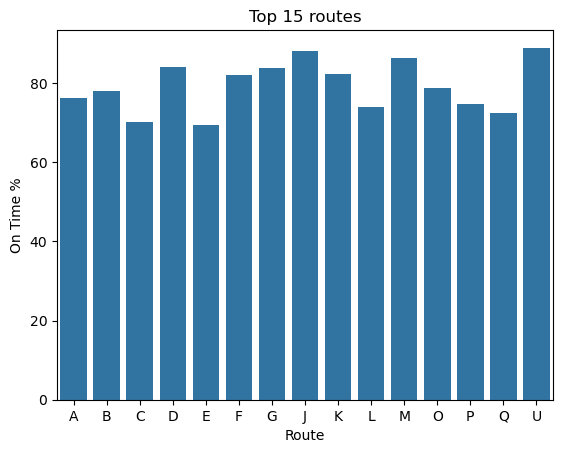
\includegraphics[width=1\linewidth]{figs/fig1.png}
		\caption[Figure 1]{Top 15 Routes}
	\end{figure}
	\begin{figure}[H]
		\centering
		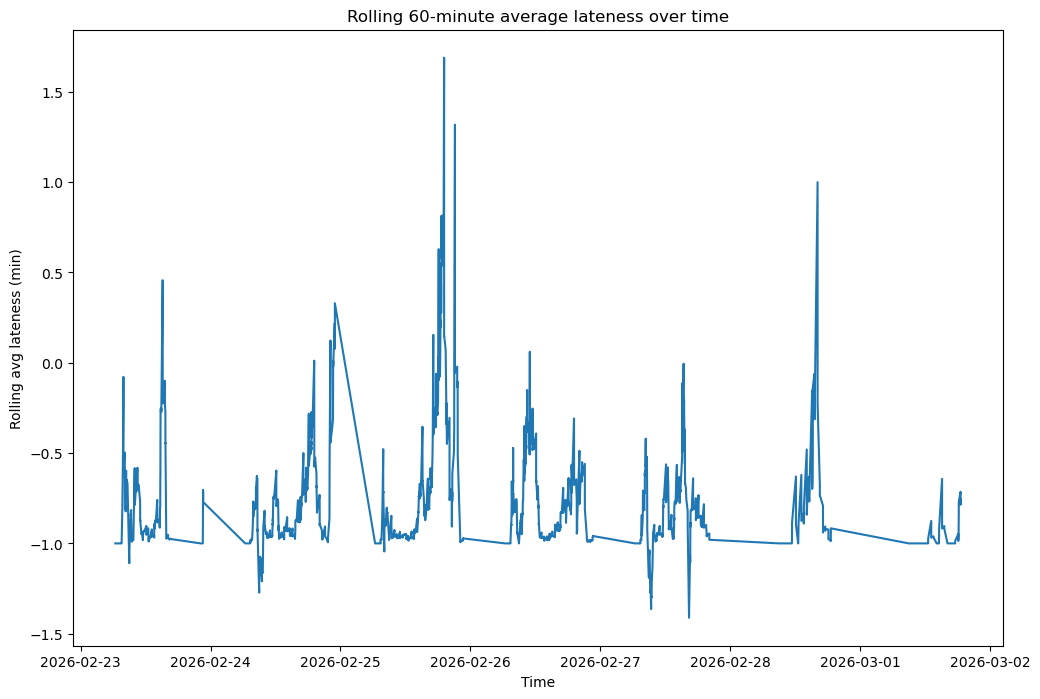
\includegraphics[width=1\linewidth]{figs/fig2.png}
		\caption[Figure 2]{Rolling 60-minutes Average Lateness Over Time}
	\end{figure}
	\begin{figure}[H]
		\centering
		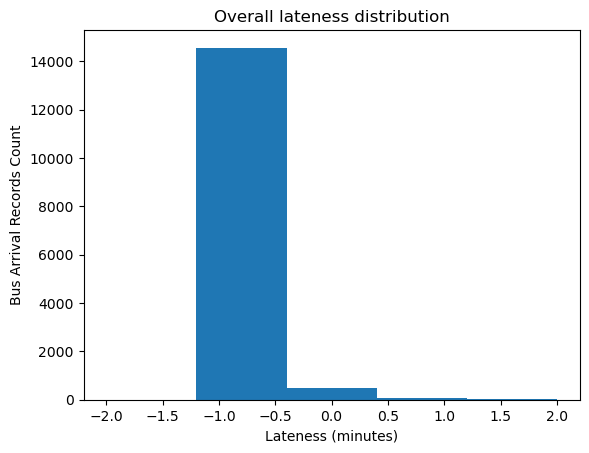
\includegraphics[width=1\linewidth]{figs/fig3.png}
		\caption[Figure 3]{Overall Lateness Distribution}
	\end{figure}
	\begin{figure}[H]
		\centering
		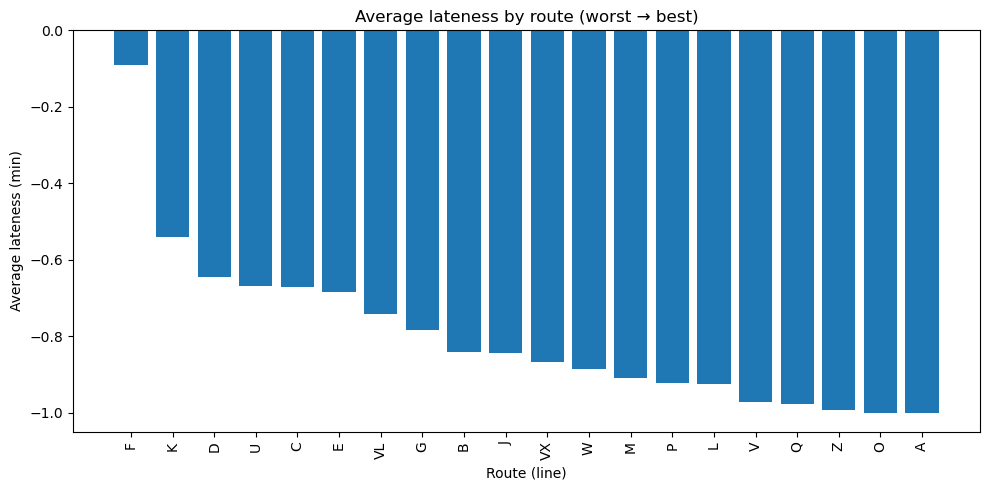
\includegraphics[width=1\linewidth]{figs/fig4.png}
		\caption[Figure 4]{Average Lateness by Route (Worst $\rightarrow$ Best)}
	\end{figure}
	\begin{figure}[H]
		\centering
		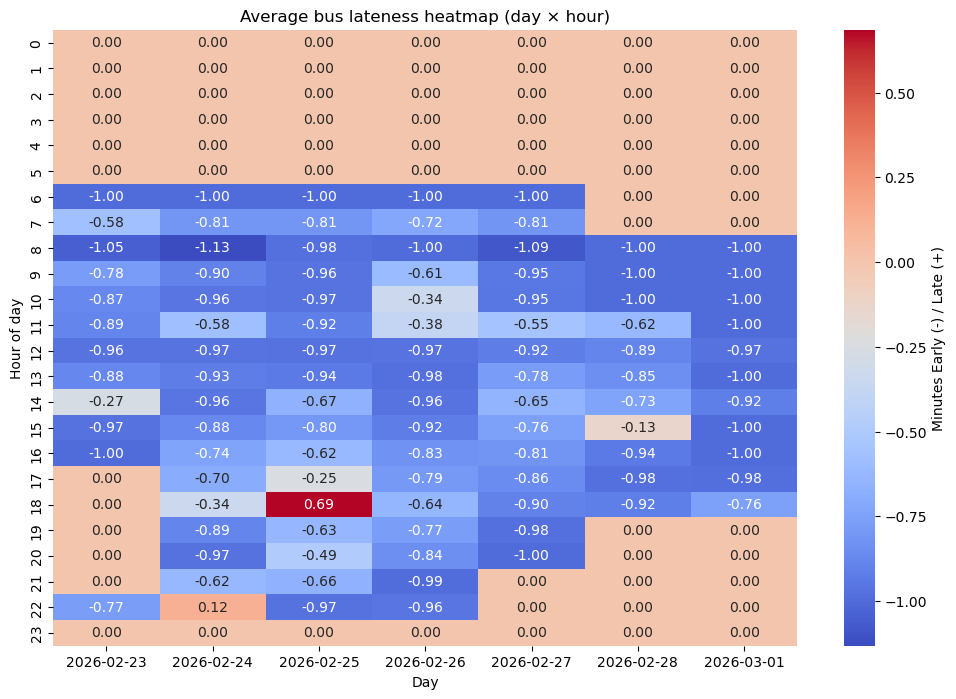
\includegraphics[width=1\linewidth]{figs/fig5.png}
		\caption[Figure 5]{Average Bus Lateness Heatmap (Day $\times$ Hour)}
	\end{figure}
	\begin{figure}[H]
		\centering
		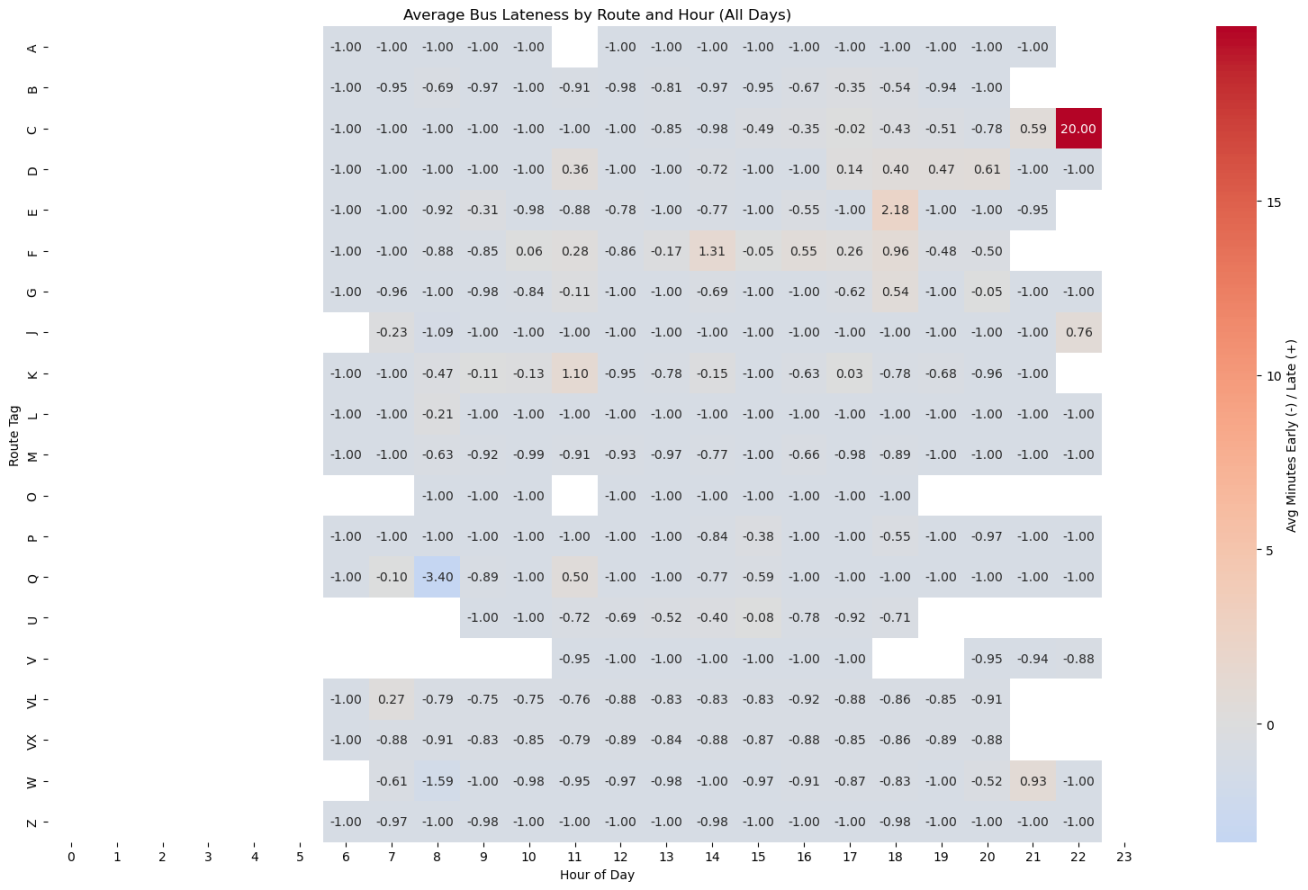
\includegraphics[width=1\linewidth]{figs/fig6.png}
		\caption[Figure 6]{Average Bus Lateness by Route and Hour (All Days)}
	\end{figure}
	\begin{figure}[H]
		\centering
		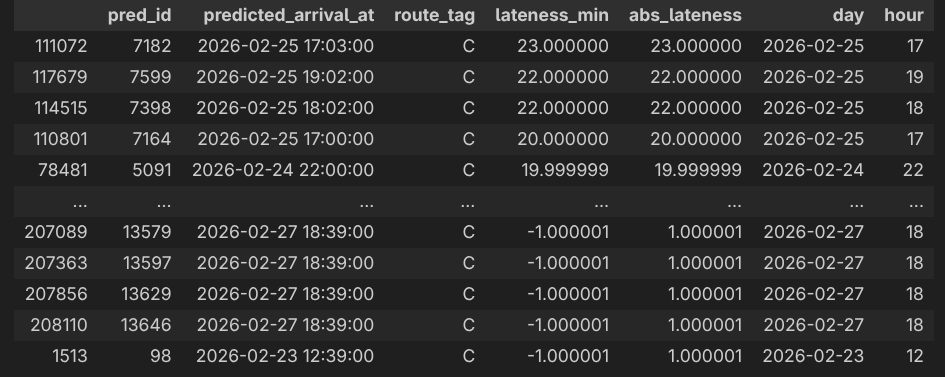
\includegraphics[width=1\linewidth]{figs/fig7.png}
		\caption[Figure 7]{C Line Data Validation}
	\end{figure}
\end{document}          
